\documentclass{article}
\usepackage{fancyhdr}
\usepackage{titlesec}
\usepackage{graphicx}
\graphicspath{ {./img/} }
\usepackage{multirow}

\pagestyle{fancy}
\fancyhf{}
\lhead{Modul 8 Praktikum Jaringan Komputer}
\rfoot{\footnotesize Page \thepage}
\lfoot{\footnotesize Mahyus Ihsan, S.Si, M.Si \newline Jurusan Informatika Universitas Syiah Kuala \newline Modul oleh : Diky Wahyudi, Furqan Al Ghifari, Rendika Rahmaturrizki}
\renewcommand{\headrulewidth}{1pt}
\renewcommand{\footrulewidth}{1pt}

\titleformat*{\section}{\small\bfseries}

\begin{document}
    \begin{center}
        \textbf{Modul 8 Praktikum Jaringan Komputer}

        \textbf{Network Security Fundamental}
    \end{center}

    \section*{Deskripsi Singkat}
    Keamanan jaringan (network security) terdiri dari kebijakan dan praktik untuk mencegah dan memantau akses yang tidak sah, penyalahgunaan, maupun penolakan yang terjadi di jaringan komputer.

Network security melibatkan otorisasi akses ke data di dalam jaringan, yang dikendalikan oleh administrator jaringan. Pengguna (users) memilih atau diberi ID dan password atau informasi otentikasi lain yang memungkinkan mereka untuk mengakses informasi dan program dalam wewenang mereka sendiri.

    \section*{Tujuan}
    \begin{enumerate}
        \item Dapat memahami ancaman dan kerentanan dalam jaringan
        \item Dapat memahami jenis-jenis serangan cyber
        \item Dapat melakukan konfigurasi firewall 
    \end{enumerate}

    \begin{flushleft}
        \textbf{Materi 1 - Ancaman dan Kerentanan dalam Jaringan}
        \newline

        Ancaman yang ada dalam jaringan 
        \begin{enumerate}
            \item Information Theft \newline
            Adalah pencurian informasi yang dilakukan dengan mencuri informasi dan menggunakan informasi tersebut untuk memperoleh keuntungan.

            \item Data loss and manipulation \newline
            Adalah kehilangan data atau manipulasi data yang disebabkan pleh pihak ketiga yang bertujuan untuk memperoleh keuntungan dari suatu pihak.

            \item Identity Theft \newline
            Identity theft atau pencurian identitas adalah kejahatan yang dilakukan dengan menyalahgunakan identitas orang lain untuk memperoleh keuntungan.

            \item Disruption of Service (DoS) \newline
            Denial-of-Service (serangan DoS) adalah serangan dunia maya di mana pelaku berupaya membuat mesin atau sumber daya jaringan tidak tersedia bagi pengguna yang dituju dengan mengganggu layanan host yang terhubung ke Internet untuk sementara atau tanpa batas.
        \end{enumerate}
    \end{flushleft}

    \newpage
    \begin{flushleft}
        \textbf{Materi 2 - Jenis - jenis Serangan Cyber}
        \newline

        Jenis - jenis serangan cyber
        \begin{enumerate}
            \item Malware \newline
            Malware adalah perangkat lunak yang dibuat dengan tujuan memasuki dan terkadang merusak sistem komputer, jaringan, atau server tanpa diketahui oleh pemiliknya.

            Contoh Malware
            \begin{enumerate}
                \item Viruses
                \item Worms
                \item Trojan Horses
            \end{enumerate}

            \item Reconnaissance Attacks \newline
            Reconnaissance Attacks adalah serangan yang berusaha untuk pengumpulan informasi dari target.

            Contoh Reconnaissance Attacks
            \begin{enumerate}
                \item Internet Queries
                \item Ping Sweeps
                \item Port Scans
            \end{enumerate}

            \item Access Attacks \newline
            Access Attacks adalah serangan yang berusahan untuk mendapatkan akses dari berbagai sumber daya data/informasi.

            Contoh Access Attacks
            \begin{enumerate}
                \item Password Attacks
                \begin{itemize}
                    \item Brute-force attacks
                    \item Trojan horse attacks
                    \item Packet sniffers
                \end{itemize}

                \item Trust Exploitation
                \item Port Redirection
                \item Man-in-the-Middle
            \end{enumerate}

            \item Denial of Service Attacks \newline
            Denial of Service Attacks adalah serangan yang menghambat penyedia layanan dengan cara mengganggu layanan komputer.

            Contoh Denial of Service Attacks
            \begin{enumerate}
                \item DoS Attack
                \item DDoS Attack
            \end{enumerate}
        \end{enumerate}
    \end{flushleft}

    \newpage
    \begin{flushleft}
        \textbf{Materi 3 - Konfigurasi Firewall dan Pembatasan Akses}
        \newline

        \begin{enumerate}
            \item Buatlah jaringan seperti gambar berikut

            \begin{center}
                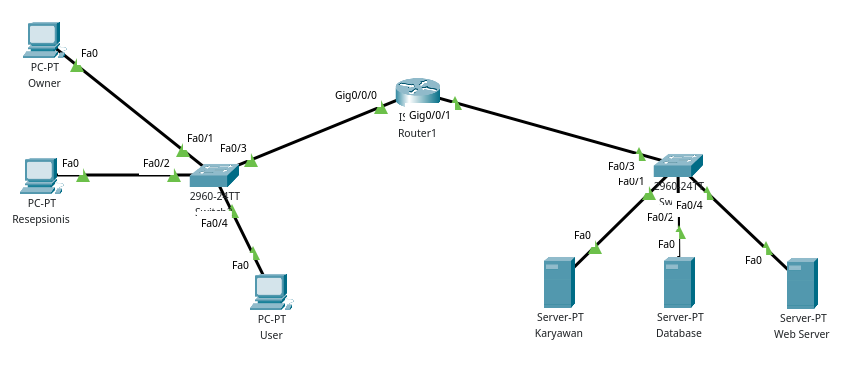
\includegraphics[scale=0.4]{3-1.png}
            \end{center}

            \begin{tabular}{|c|c|c|c|c|}
                \hline
                Device & IP & Dest & Network & Gateway \\
                \hline
                \multirow{2}{4em}{Router0} & 192.168.1.1 & Switch0 & 192.168.1.0/29 & - \\
                & 192.168.1.9 & Switch1 & 192.168.1.8/29 & - \\
                \hline
                Owner & 192.168.1.2 & - & 192.168.1.0/29 & 192.168.1.1\\
                \hline
                Resepsionis & 192.168.1.3 & - & 192.168.1.0/29 & 192.168.1.1\\
                \hline
                User & 192.168.1.4 & - & 192.168.1.0/29 & 192.168.1.1\\
                \hline
                Karyawan & 192.168.1.10 & - & 192.168.1.8/29 & 192.168.1.9\\
                \hline
                Database & 192.168.1.11 & - & 192.168.1.8/29 & 192.168.1.9\\
                \hline
                Web Server & 192.168.1.12 & - & 192.168.1.8/29 & 192.168.1.9\\
                \hline
            \end{tabular}

            \item Coba lakukan ping dari PC Owner , Resepsionis dan User ke masing - masing server, apakah semua device bisa mengakses semua server yang ada ?
            
            \item Selanjutnya kita akan membatasi aksek server Karyawan agar bisa di akses oleh Owner saja. Buka Server Karyawan dan buka menu \textbf{Desktop $>$ Firewall}
            
            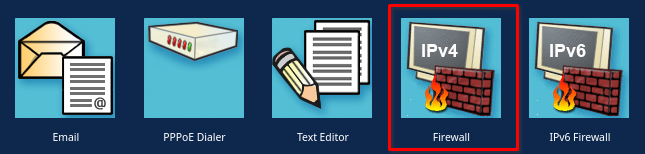
\includegraphics[scale=0.6]{3-2.png}

            \item Kemudian berikan PC Owner akses ke server Karyawan dan otomatis selain dari owner tidak akan bisa mengakses server karyawan.
            
            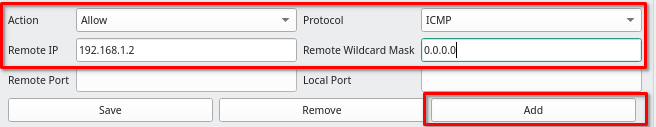
\includegraphics[scale=0.6]{3-3.png}

            \item Setelah berhasil ditambahkan , silahkan lakukan ping dari PC Owner ke server karyawan dan lakukan juga ping dari PC Resepsionis dan User. Maka yang berhasil 
            
            \begin{center}
                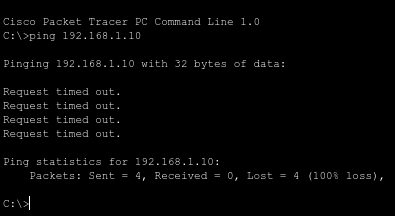
\includegraphics[]{3-4.png}

                Ping menggunakan PC User
            \end{center}
            
            \begin{center}
                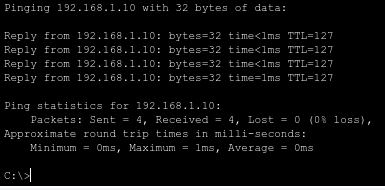
\includegraphics[]{3-5.png}

                Ping menggunakan PC Owner
            \end{center}

            \item Kemudian pada server Database tambahkan PC Owner dan PC Resepsionis agar hanya PC Owner dan Resepsionis yang dapat mengakses server Database sedangkan PC User tidak bisa.
            
            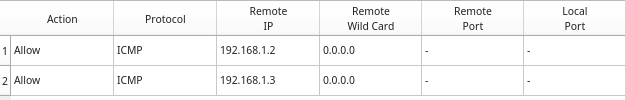
\includegraphics[scale=0.6]{3-6.png}
            
            \item Kemudian tambahkan 2 buah PC dan lakukan konfigurasi pada kedua pc tersebut

            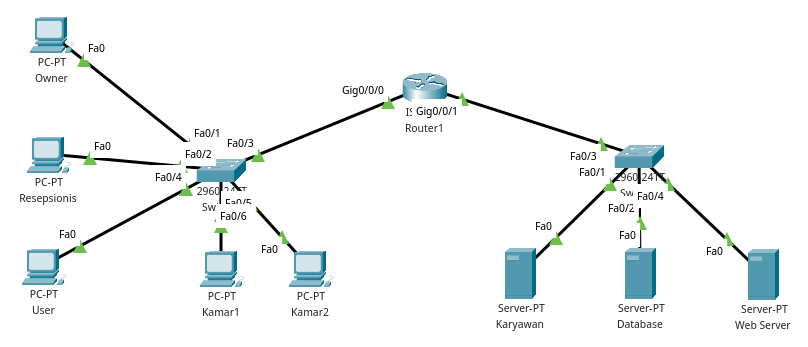
\includegraphics[scale=0.5]{3-7.png}

            \item Kemudian kita akan membatasi akses PC Kamar1 dan Kamar2 agar tidak bisa mengakses jaringan luar
            
            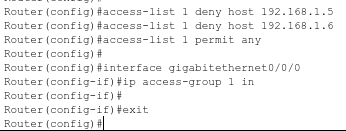
\includegraphics[scale=1.1]{3-8.png}

            Penjelasan
            \begin{itemize}
                \item access-list 1 deny host 192.168.1.5 untuk membatasi akses pc dengan ip 192.168.1.5
                \item access-list 1 permit any untuk memberi akses kepada seluruh host kecuali yang masuk kedalam list deny tadi
                \item ip access-group 1 in untuk memasukkan access-group kedalam interface yang dipilih
            \end{itemize}

            \item Kemudian lakukan ping pada PC Kamar1 dan Kamar 2 maka akan muncul pesan seperti berikut, sedangkan PC lainnya bisa untuk mengakses jaringan diluar dari jaringan mereka

            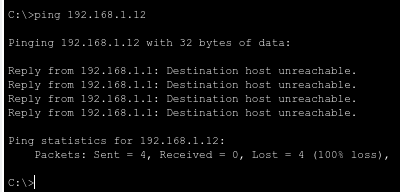
\includegraphics[scale=0.7]{3-9.png}
        \end{enumerate}
    \end{flushleft}
\end{document}
